%sage: G = Graph([[1,2],[2,3],[3,4]])                                                                                                                                                                      
%sage: GP = GraphicalPolytopes(G)                                                                                                                                                                          
%sage: CP = GP.chunk_polytope(tuple([]), tuple([]), weights=GP.standard_weights(), essential=True)                                                                                                         
%sage: to_tikz(CP, nb=True)                                                                                                                                                                                

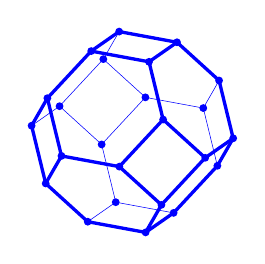
\begin{tikzpicture}%
	[x={(-0.366215cm, -0.789554cm)},
	y={(0.235950cm, -0.590693cm)},
	z={(0.900119cm, -0.166391cm)},
	scale=.5,
	back/.style={very thin},
	edge/.style={color=blue, very thick},
	facet/.style={fill=blue,fill opacity=0},
	vertex/.style={inner sep=1pt,circle,fill=blue,thick},
	baseline=0]

%% Coordinate of the vertices:
%%
\coordinate (-2.00000, -1.41421, -0.81650) at (-2.00000, -1.41421, -0.81650);
\coordinate (-2.00000, -1.41421, 0.81650) at (-2.00000, -1.41421, 0.81650);
\coordinate (-2.00000, 0.00000, -1.63299) at (-2.00000, 0.00000, -1.63299);
\coordinate (-2.00000, 0.00000, 1.63299) at (-2.00000, 0.00000, 1.63299);
\coordinate (-2.00000, 1.41421, -0.81650) at (-2.00000, 1.41421, -0.81650);
\coordinate (-2.00000, 1.41421, 0.81650) at (-2.00000, 1.41421, 0.81650);
\coordinate (-0.66667, -2.35702, -0.81650) at (-0.66667, -2.35702, -0.81650);
\coordinate (-0.66667, -2.35702, 0.81650) at (-0.66667, -2.35702, 0.81650);
\coordinate (-0.66667, 0.47140, -2.44949) at (-0.66667, 0.47140, -2.44949);
\coordinate (-0.66667, 0.47140, 2.44949) at (-0.66667, 0.47140, 2.44949);
\coordinate (-0.66667, 1.88562, -1.63299) at (-0.66667, 1.88562, -1.63299);
\coordinate (-0.66667, 1.88562, 1.63299) at (-0.66667, 1.88562, 1.63299);
\coordinate (0.66667, -1.88562, -1.63299) at (0.66667, -1.88562, -1.63299);
\coordinate (0.66667, -1.88562, 1.63299) at (0.66667, -1.88562, 1.63299);
\coordinate (0.66667, -0.47140, -2.44949) at (0.66667, -0.47140, -2.44949);
\coordinate (0.66667, -0.47140, 2.44949) at (0.66667, -0.47140, 2.44949);
\coordinate (0.66667, 2.35702, -0.81650) at (0.66667, 2.35702, -0.81650);
\coordinate (0.66667, 2.35702, 0.81650) at (0.66667, 2.35702, 0.81650);
\coordinate (2.00000, -1.41421, -0.81650) at (2.00000, -1.41421, -0.81650);
\coordinate (2.00000, -1.41421, 0.81650) at (2.00000, -1.41421, 0.81650);
\coordinate (2.00000, 0.00000, -1.63299) at (2.00000, 0.00000, -1.63299);
\coordinate (2.00000, 0.00000, 1.63299) at (2.00000, 0.00000, 1.63299);
\coordinate (2.00000, 1.41421, -0.81650) at (2.00000, 1.41421, -0.81650);
\coordinate (2.00000, 1.41421, 0.81650) at (2.00000, 1.41421, 0.81650);
%%
%%
%% Drawing edges in the back
%%
\draw[edge,back] (-2.00000, -1.41421, -0.81650) -- (-2.00000, 0.00000, -1.63299);
\draw[edge,back] (-2.00000, 0.00000, -1.63299) -- (-2.00000, 1.41421, -0.81650);
\draw[edge,back] (-2.00000, 0.00000, -1.63299) -- (-0.66667, 0.47140, -2.44949);
\draw[edge,back] (-2.00000, 0.00000, 1.63299) -- (-2.00000, 1.41421, 0.81650);
\draw[edge,back] (-2.00000, 1.41421, -0.81650) -- (-2.00000, 1.41421, 0.81650);
\draw[edge,back] (-2.00000, 1.41421, -0.81650) -- (-0.66667, 1.88562, -1.63299);
\draw[edge,back] (-2.00000, 1.41421, 0.81650) -- (-0.66667, 1.88562, 1.63299);
\draw[edge,back] (-0.66667, 0.47140, -2.44949) -- (-0.66667, 1.88562, -1.63299);
\draw[edge,back] (-0.66667, 0.47140, -2.44949) -- (0.66667, -0.47140, -2.44949);
\draw[edge,back] (-0.66667, 1.88562, -1.63299) -- (0.66667, 2.35702, -0.81650);
\draw[edge,back] (0.66667, 2.35702, -0.81650) -- (0.66667, 2.35702, 0.81650);
\draw[edge,back] (0.66667, 2.35702, -0.81650) -- (2.00000, 1.41421, -0.81650);
%%
%%
%% Drawing vertices in the back
%%
\node[vertex] at (-0.66667, 0.47140, -2.44949)     {};
\node[vertex] at (-0.66667, 1.88562, -1.63299)     {};
\node[vertex] at (0.66667, 2.35702, -0.81650)     {};
\node[vertex] at (-2.00000, 0.00000, -1.63299)     {};
\node[vertex] at (-2.00000, 1.41421, -0.81650)     {};
\node[vertex] at (-2.00000, 1.41421, 0.81650)     {};
%%
%%
%% Drawing the facets
%%
\fill[facet] (2.00000, 0.00000, -1.63299) -- (0.66667, -0.47140, -2.44949) -- (0.66667, -1.88562, -1.63299) -- (2.00000, -1.41421, -0.81650) -- cycle {};
\fill[facet] (-0.66667, -2.35702, 0.81650) -- (-2.00000, -1.41421, 0.81650) -- (-2.00000, -1.41421, -0.81650) -- (-0.66667, -2.35702, -0.81650) -- cycle {};
\fill[facet] (0.66667, -0.47140, 2.44949) -- (-0.66667, 0.47140, 2.44949) -- (-2.00000, 0.00000, 1.63299) -- (-2.00000, -1.41421, 0.81650) -- (-0.66667, -2.35702, 0.81650) -- (0.66667, -1.88562, 1.63299) -- cycle {};
\fill[facet] (2.00000, -1.41421, 0.81650) -- (0.66667, -1.88562, 1.63299) -- (-0.66667, -2.35702, 0.81650) -- (-0.66667, -2.35702, -0.81650) -- (0.66667, -1.88562, -1.63299) -- (2.00000, -1.41421, -0.81650) -- cycle {};
\fill[facet] (2.00000, 0.00000, 1.63299) -- (0.66667, -0.47140, 2.44949) -- (0.66667, -1.88562, 1.63299) -- (2.00000, -1.41421, 0.81650) -- cycle {};
\fill[facet] (2.00000, 1.41421, 0.81650) -- (0.66667, 2.35702, 0.81650) -- (-0.66667, 1.88562, 1.63299) -- (-0.66667, 0.47140, 2.44949) -- (0.66667, -0.47140, 2.44949) -- (2.00000, 0.00000, 1.63299) -- cycle {};
\fill[facet] (2.00000, 1.41421, 0.81650) -- (2.00000, 0.00000, 1.63299) -- (2.00000, -1.41421, 0.81650) -- (2.00000, -1.41421, -0.81650) -- (2.00000, 0.00000, -1.63299) -- (2.00000, 1.41421, -0.81650) -- cycle {};
%%
%%
%% Drawing edges in the front
%%
\draw[edge] (-2.00000, -1.41421, -0.81650) -- (-2.00000, -1.41421, 0.81650);
\draw[edge] (-2.00000, -1.41421, -0.81650) -- (-0.66667, -2.35702, -0.81650);
\draw[edge] (-2.00000, -1.41421, 0.81650) -- (-2.00000, 0.00000, 1.63299);
\draw[edge] (-2.00000, -1.41421, 0.81650) -- (-0.66667, -2.35702, 0.81650);
\draw[edge] (-2.00000, 0.00000, 1.63299) -- (-0.66667, 0.47140, 2.44949);
\draw[edge] (-0.66667, -2.35702, -0.81650) -- (-0.66667, -2.35702, 0.81650);
\draw[edge] (-0.66667, -2.35702, -0.81650) -- (0.66667, -1.88562, -1.63299);
\draw[edge] (-0.66667, -2.35702, 0.81650) -- (0.66667, -1.88562, 1.63299);
\draw[edge] (-0.66667, 0.47140, 2.44949) -- (-0.66667, 1.88562, 1.63299);
\draw[edge] (-0.66667, 0.47140, 2.44949) -- (0.66667, -0.47140, 2.44949);
\draw[edge] (-0.66667, 1.88562, 1.63299) -- (0.66667, 2.35702, 0.81650);
\draw[edge] (0.66667, -1.88562, -1.63299) -- (0.66667, -0.47140, -2.44949);
\draw[edge] (0.66667, -1.88562, -1.63299) -- (2.00000, -1.41421, -0.81650);
\draw[edge] (0.66667, -1.88562, 1.63299) -- (0.66667, -0.47140, 2.44949);
\draw[edge] (0.66667, -1.88562, 1.63299) -- (2.00000, -1.41421, 0.81650);
\draw[edge] (0.66667, -0.47140, -2.44949) -- (2.00000, 0.00000, -1.63299);
\draw[edge] (0.66667, -0.47140, 2.44949) -- (2.00000, 0.00000, 1.63299);
\draw[edge] (0.66667, 2.35702, 0.81650) -- (2.00000, 1.41421, 0.81650);
\draw[edge] (2.00000, -1.41421, -0.81650) -- (2.00000, -1.41421, 0.81650);
\draw[edge] (2.00000, -1.41421, -0.81650) -- (2.00000, 0.00000, -1.63299);
\draw[edge] (2.00000, -1.41421, 0.81650) -- (2.00000, 0.00000, 1.63299);
\draw[edge] (2.00000, 0.00000, -1.63299) -- (2.00000, 1.41421, -0.81650);
\draw[edge] (2.00000, 0.00000, 1.63299) -- (2.00000, 1.41421, 0.81650);
\draw[edge] (2.00000, 1.41421, -0.81650) -- (2.00000, 1.41421, 0.81650);
%%
%%
%% Drawing the vertices in the front
%%
\node[vertex] at (-2.00000, -1.41421, -0.81650)     {};
\node[vertex] at (-2.00000, -1.41421, 0.81650)     {};
\node[vertex] at (-2.00000, 0.00000, 1.63299)     {};
\node[vertex] at (-0.66667, -2.35702, -0.81650)     {};
\node[vertex] at (-0.66667, -2.35702, 0.81650)     {};
\node[vertex] at (-0.66667, 0.47140, 2.44949)     {};
\node[vertex] at (-0.66667, 1.88562, 1.63299)     {};
\node[vertex] at (0.66667, -1.88562, -1.63299)     {};
\node[vertex] at (0.66667, -1.88562, 1.63299)     {};
\node[vertex] at (0.66667, -0.47140, -2.44949)     {};
\node[vertex] at (0.66667, -0.47140, 2.44949)     {};
\node[vertex] at (0.66667, 2.35702, 0.81650)     {};
\node[vertex] at (2.00000, -1.41421, -0.81650)     {};
\node[vertex] at (2.00000, -1.41421, 0.81650)     {};
\node[vertex] at (2.00000, 0.00000, -1.63299)     {};
\node[vertex] at (2.00000, 0.00000, 1.63299)     {};
\node[vertex] at (2.00000, 1.41421, -0.81650)     {};
\node[vertex] at (2.00000, 1.41421, 0.81650)     {};
%%
%%
\end{tikzpicture}